\section{Results and Discussion}

The classification results are shown in Figure \ref{fig:kappa}. Higher kappa values indicate better classification performance. A kappa value $k=0$ indicates a random decision. According to Figure \ref{fig:kappa}, a higher classification performance is achieved with Nonlinear Regression Analysis compared to Granger's causality. In order to investigate if the kappa values are significantly non-random, a one-way \emph{Student-t test} is applied for each case. The null hypothesis is that the kappa values for each case follow a Student distribution with zero mean. The null hypothesis is rejected for the case of Nonlinear Regression Analysis ($p<0.05$, $\kappa$ values with $\mu = 0.07, median = 0.06,\sigma = 0.17$). Although this value is statistically significant, it is still close to zero. However, 14 out of 23 subjects have kappa values larger than zero. The null hypothesis is not rejected for the Granger causality case. This finding indicates that nonlinear patterns occur in the functional connectivity of neural assemblies, able to discriminate between pleasant and unpleasant odours. 

\begin{figure}[t]
    \centering
    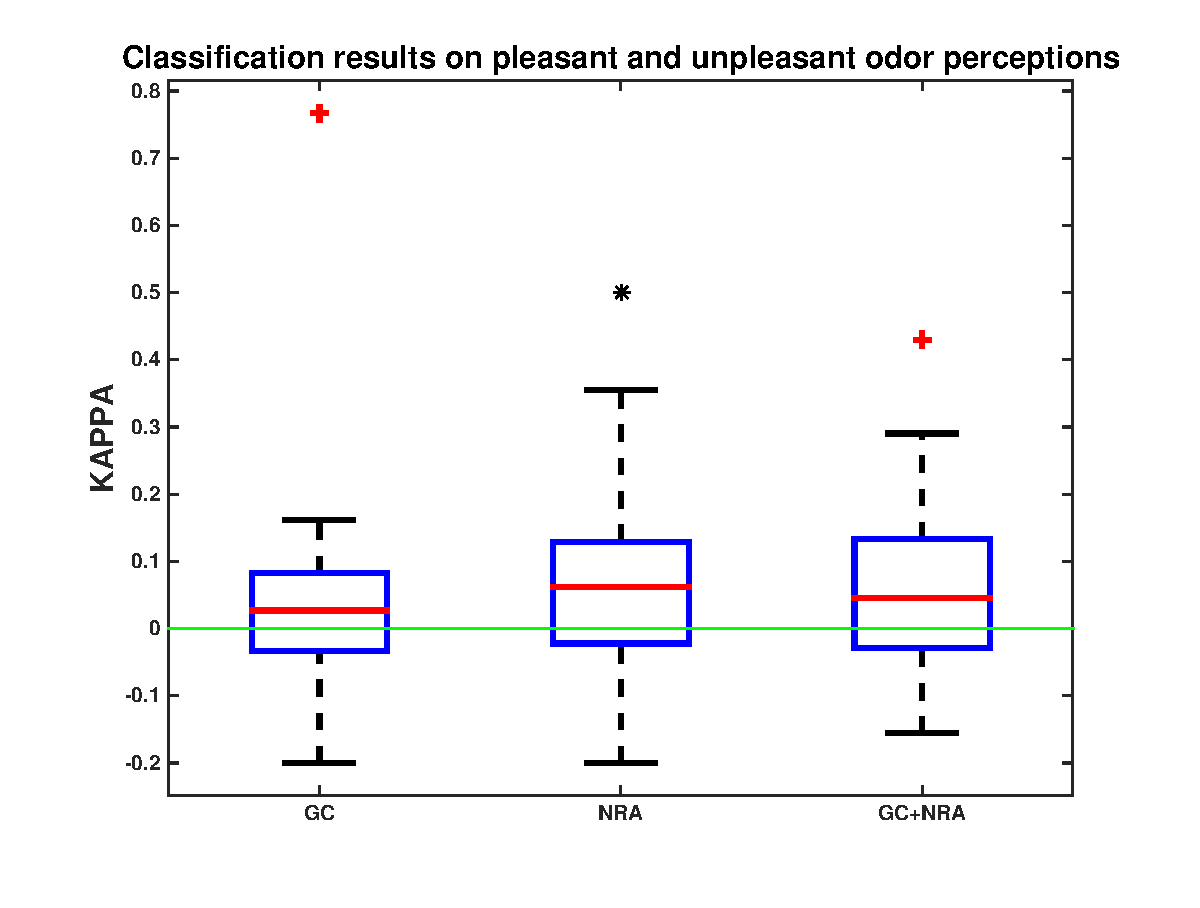
\includegraphics[width=0.45\textwidth]{./images/kappa.eps}
    \caption{Cohen's Kappa resluts boxplots. On each box, the central (red) line represents the median value, the upside and downside edges represent the 25th and 75th percentiles, and the red crosses represent outliers. The green line represents the random decision, $Kappa=0$. GC refers to the kappa values estimated for features extracted from the networks estimated using Granger Causality. NRA refers to the kappa values estimated for features extracted from the networks estimated using Nonlinear Regression Analysis. GC+NRA refers to the kappa values estimated using features both from Granger Causality and from Nonlinear Regression Analysis methods.}
    \label{fig:kappa}
\end{figure}

In order to investigate the classification performance of the two feature-categories, namely the small-world network features and the free-scale network features, a SVM classifier is trained and tested as previously, for each feature-category. The results are presented in Figure \ref{fig:feat_category}. In order to investigate if each feature-category leads to significantly non-random kappa values, a one-way \emph{Student-t test} is applied as previously. The results reveal that the small-world network features lead to a significantly non-random performance, whereas this is not the case for the free-scale network features. This finding indicates that odour pleasantness perception can be depicted in small-world network features extracted from the functional connectivity across neural assemblies which is estimated using Nonlinear Regression Analysis. 

%%%%%%%%%%%%%%%%%%%%%%%%%%%%%%%%%%%%%%%%%%%%%%%%%%%%%%%%%%%%%%%%%%%%%%%%%%%%%%
%%                             TABLE 1
%%%%%%%%%%%%%%%%%%%%%%%%%%%%%%%%%%%%%%%%%%%%%%%%%%%%%%%%%%%%%%%%%%%%%%%%%%%%%%
\begin{table}[ht]
\caption{Kappa descriptives for each classification scenario. Min stands for minimum kappa value, max for maximum kappa value, and SD for standard deviation. The asterisks indicate significance with $p<0.05$.}\label{Table1}
\centering % for placing the table in the middle of the page
{\begin{tabular}{|l|c|c|c|c|}
\hline
\toprule
 \textbf{Features} & \textbf{Min} & \textbf{Max} & \textbf{Mean} & \textbf{SD}\\
\hline
\toprule
\textbf{GC} & 0.57 & 0 & 0.43 & \\
\hline
\toprule
 \textbf{NRA} & 0 & 1 & 0 & \\
\hline
\toprule
\textbf{GC+NRA} & 0.58 & 0 & 0.42 & \\
\hline
\toprule
\textbf{Small-world} & 0.57 & 0 & 0.43 & \\
\hline
\toprule
 \textbf{Free scale} & 0 & 1 & 0 & \\
\hline
\toprule
\textbf{Characteristic path**} & -0.1 & 0.45 & 0.096 & 0.15\\
\hline
\toprule
\textbf{Local efficiency**} & -0.14 & 0.37 & 0.09 & 0.14\\
\hline
\toprule
\textbf{Global efficiency**} & -0.17 & 0.5 & 0.11 & 0.17\\
\hline
\toprule
 \textbf{Clustering coefficient**} & -0.15 & 0.5 & 0.11 & 0.16\\
\hline
\toprule
\textbf{Shannon entropy} & 0 & 0 & 0.42 & \\
\hline
\toprule
\textbf{von Neumann entropy} & -0.13 & 0.3 & 0.01 & 0.12\\
\bottomrule
\end{tabular}}
%\begin{tabnote}
%SD indicates Significant Differences (with $p<0.01$), whereas NS indicates No Significant differences ($p>0.05$).
%\end{tabnote}
\end{table}
%%%%%%%%%%%%%%%%%%%%%%%%%%%%%%%%%%%%%%%%%%%%%%%%%%%%%%%%%%%%%%%%%%%%%%%%%%%%%%


Finally, in order to further explore which individual feature increases the classification performance, the same analysis as previously is carried out for each feature. The results are presented in Figure  \ref{fig:feat_indiv}. According to this figure, the global efficiency leads to the best average Kappa value $k=0.1112 \pm 0.1673$, which is significantly non-random ($p<0.01$). Table \ref{Table1} presents the kappa descriptives (min, max, mean, and standard deviation) estimated for each case. One may notice from this Table that the global efficiency extracted from the brain network estimated using Nonlinear Regression Analysis leads to the best classification performance. 


%Lower kappa value indicates that the classifier is making more random decisions (bad performance) while higher values indicates the classifier is making non-random decisions (better performance). From our kappa results we find that most classifiers' performances are not far away from random decisions ($\kappa$ <0.2 \cite{cohenskappa}). But there are still some features can help the classifier stop making random decisions. We run \emph{Student-t test} on the kappa values for each feature of each network to test the randomness of Kappa results. The t-test shows that kappa result from Nonlinear Regression Analysis features ($p = 0.0409 < 0.05$, $\kappa$ values with $\mu = 0.0628, median = 0.0573,\sigma = 0.1387$) is significantly not random. If we look inside of each features of 216-channel Nonlinear Regression Analysis functional connectivity maps, we found that  216-channel Nonlinear Regression Analysis weighted feature of \emph{global efficiency} can give the best Kappa result with significantly non-randomness ($p = 0.0043$) of $0.1112 \pm 0.1673$.

%Although the significant kappa result have a $p-values$ less than 0.05, some of the $p-values$ are still very close to 0.05, indicating that the results are not that good anyway.The low classification accuracy may due to many reasons: the size of functional connectivity map may play a crucial rule in classification -- the 216-channel functional connectivity maps may provide too much redundant information in classification. New features of functional connectivity maps should also be proposed and used for classification. Since we only used network-based features in this paper, other features as power spectral density or time-frequency analysis may also be used in combination for classification. Another improvement for getting better classification results could be done in the experiment design. Based on the experiment protocol and preprocessing of raw EEG signal, 6 seconds of each trial of EEG signal are kept fro investigating the pleasantness from odours. This time duration could be cut shorter (because 6 seconds might be to much for decision making) or extended longer (or because 6 seconds might be not enough to make the decision). Nevertheless, this paper is not targeting to replace existing methods for affective computing on emotions, but to propose a new direction for affective computing. 